\documentclass[12pt]{article}
\usepackage{amsmath}
\usepackage{amsfonts}
\usepackage{bm}
\usepackage{color}
\usepackage{graphicx}
\definecolor{lyellow}{rgb}{0.97,0.94,0.8}
\definecolor{gray}{rgb}{0.4,0.4,0.4}

%\renewcommand{\baselinestretch}{1.2}

\textwidth 15.5cm
\textheight 22.5cm
\topmargin  0.0cm
\oddsidemargin -0cm
\evensidemargin -0cm
%\pagestyle{empty}

%\partopsep -33pt
%\parsep 0pt
%\topskip -33pt
%\parskip 33pt


\newcommand{\lfrac}[2]{{\displaystyle\frac{{#1}}{{#2}}}}
\newcommand{\ffrac}[2]{{\textstyle\frac{{#1}}{{#2}}}}
\newcommand{\half}{\ffrac{1}{2}}



\newcommand{\I}{\mathrm{i}}
%\newcommand{\bld}[1]{\boldsymbol{#1}}
\newcommand{\cond}{\mbox{\rule[-0.5em]{.1mm}{1.2em}}}

%\renewcommand{\baselinestretch}{0.9}
\renewcommand{\topfraction}{0.8}
\renewcommand{\textfraction}{0.2}
\renewcommand{\floatpagefraction}{0.8}

\newcounter{denselistcounter}
\newenvironment{denselist}[1]
{ \begin{list}
  {#1{denselistcounter})}{\usecounter{denselistcounter}
  \setlength{\topsep}{-0pt}
  \setlength{\partopsep}{-0pt}
  \setlength{\itemsep}{-0pt}
  \setlength{\parsep}{-0pt}
  \setlength{\labelwidth}{6pt}
  \setlength{\labelsep}{4pt}
  \setlength{\leftmargin}{20pt}
  \setlength{\rightmargin}{20pt}
  }
}
{\end{list}}

\newcommand{\Bp}{\mathcal{B}_0}
\newcommand{\Bm}{\mathcal{B}_1}
\newcommand{\PGR}[1]{{\color{blue} #1}}

\begin{document}

\title{Finite-range pairing: the impact of width}
\author{Discussion file: FAU -- MSU}
\date{Started: 1. August 2024}
\maketitle


\bigskip

\centerline{\includegraphics[width=0.5\linewidth]{plots/PairingGap_bcs_120Sn_SVbas_Cut100}
            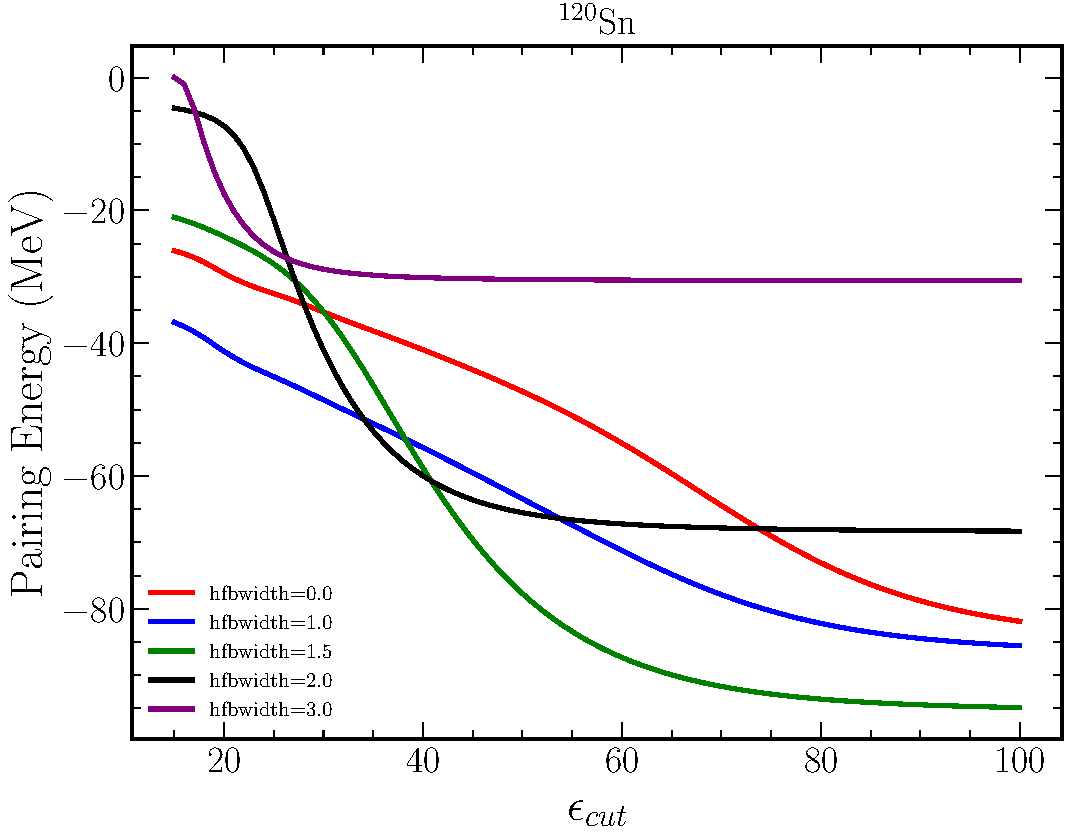
\includegraphics[width=0.5\linewidth]{plots/PairingEnergy_bcs_120Sn_SVbas_Cut100}}

\bigskip
To state the problem, we start with the above figure. It shows the
$uv$-averaged pairing gap (left) abnd pairing energy (right) as
function of the cutoff $\epsilon_\mathrm{cut}$ for four different folding widths. Test case is
neutron pairing in $^{120}$Sn computed with SV-bas and BCS
pairing. The trends are the same for other nuclei, functionals, and
HFB. Pairing strength are calibrated to yield the same averge gap at
the largest cutoff  $\epsilon_\mathrm{cut}=100$ MeV. 

We expect faster convergence with $\epsilon_\mathrm{cut}$ for
increasing width. This seem to be given. Nonetheless, the results are
puzzling. The group of widths 0 and 1 fm behaves much diifferent from
the group of widths 2 and 3 fm. From 0 fm up to 1.5 fm (not shown
here), there are monotoneous trends. Above 1.5 fm, i.e. for widths 2
and 3 fm, the trends are reverted. Somewhat surprisingly, the larger
widths undergo larger changes and show even a pairing break-down
toward small  $\epsilon_\mathrm{cut}$. This is disquiteing as it
indicates that widths above 1.5 fm are unsafe to use.

To understand what is going on, we investigate the behavior in more detail.


\bigskip

\centerline{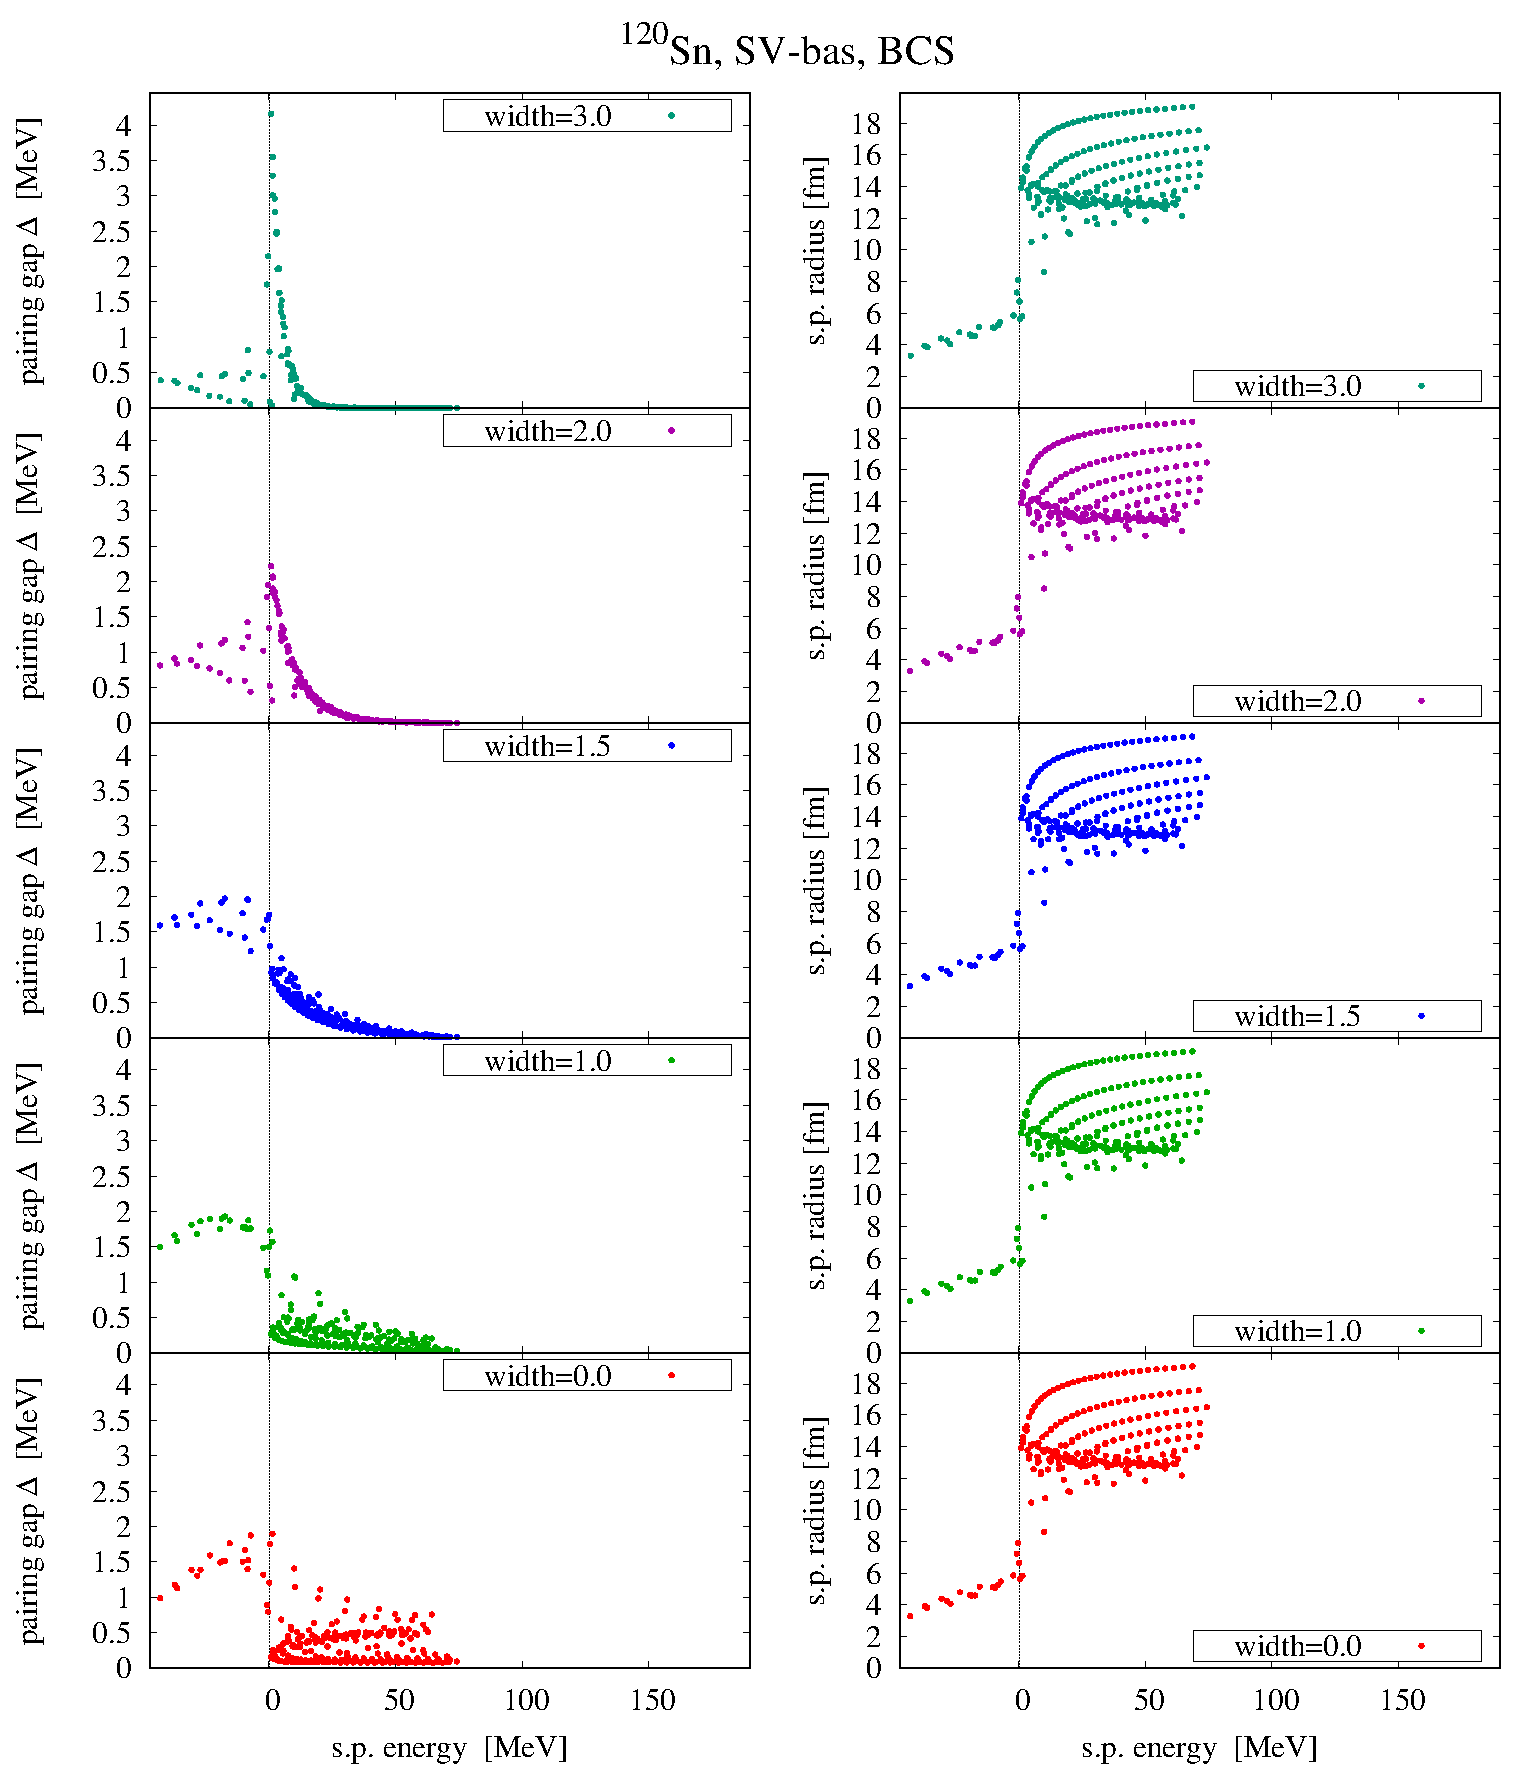
\includegraphics[width=0.8\linewidth]{varywid_BCS}}

\bigskip



\bigskip

\centerline{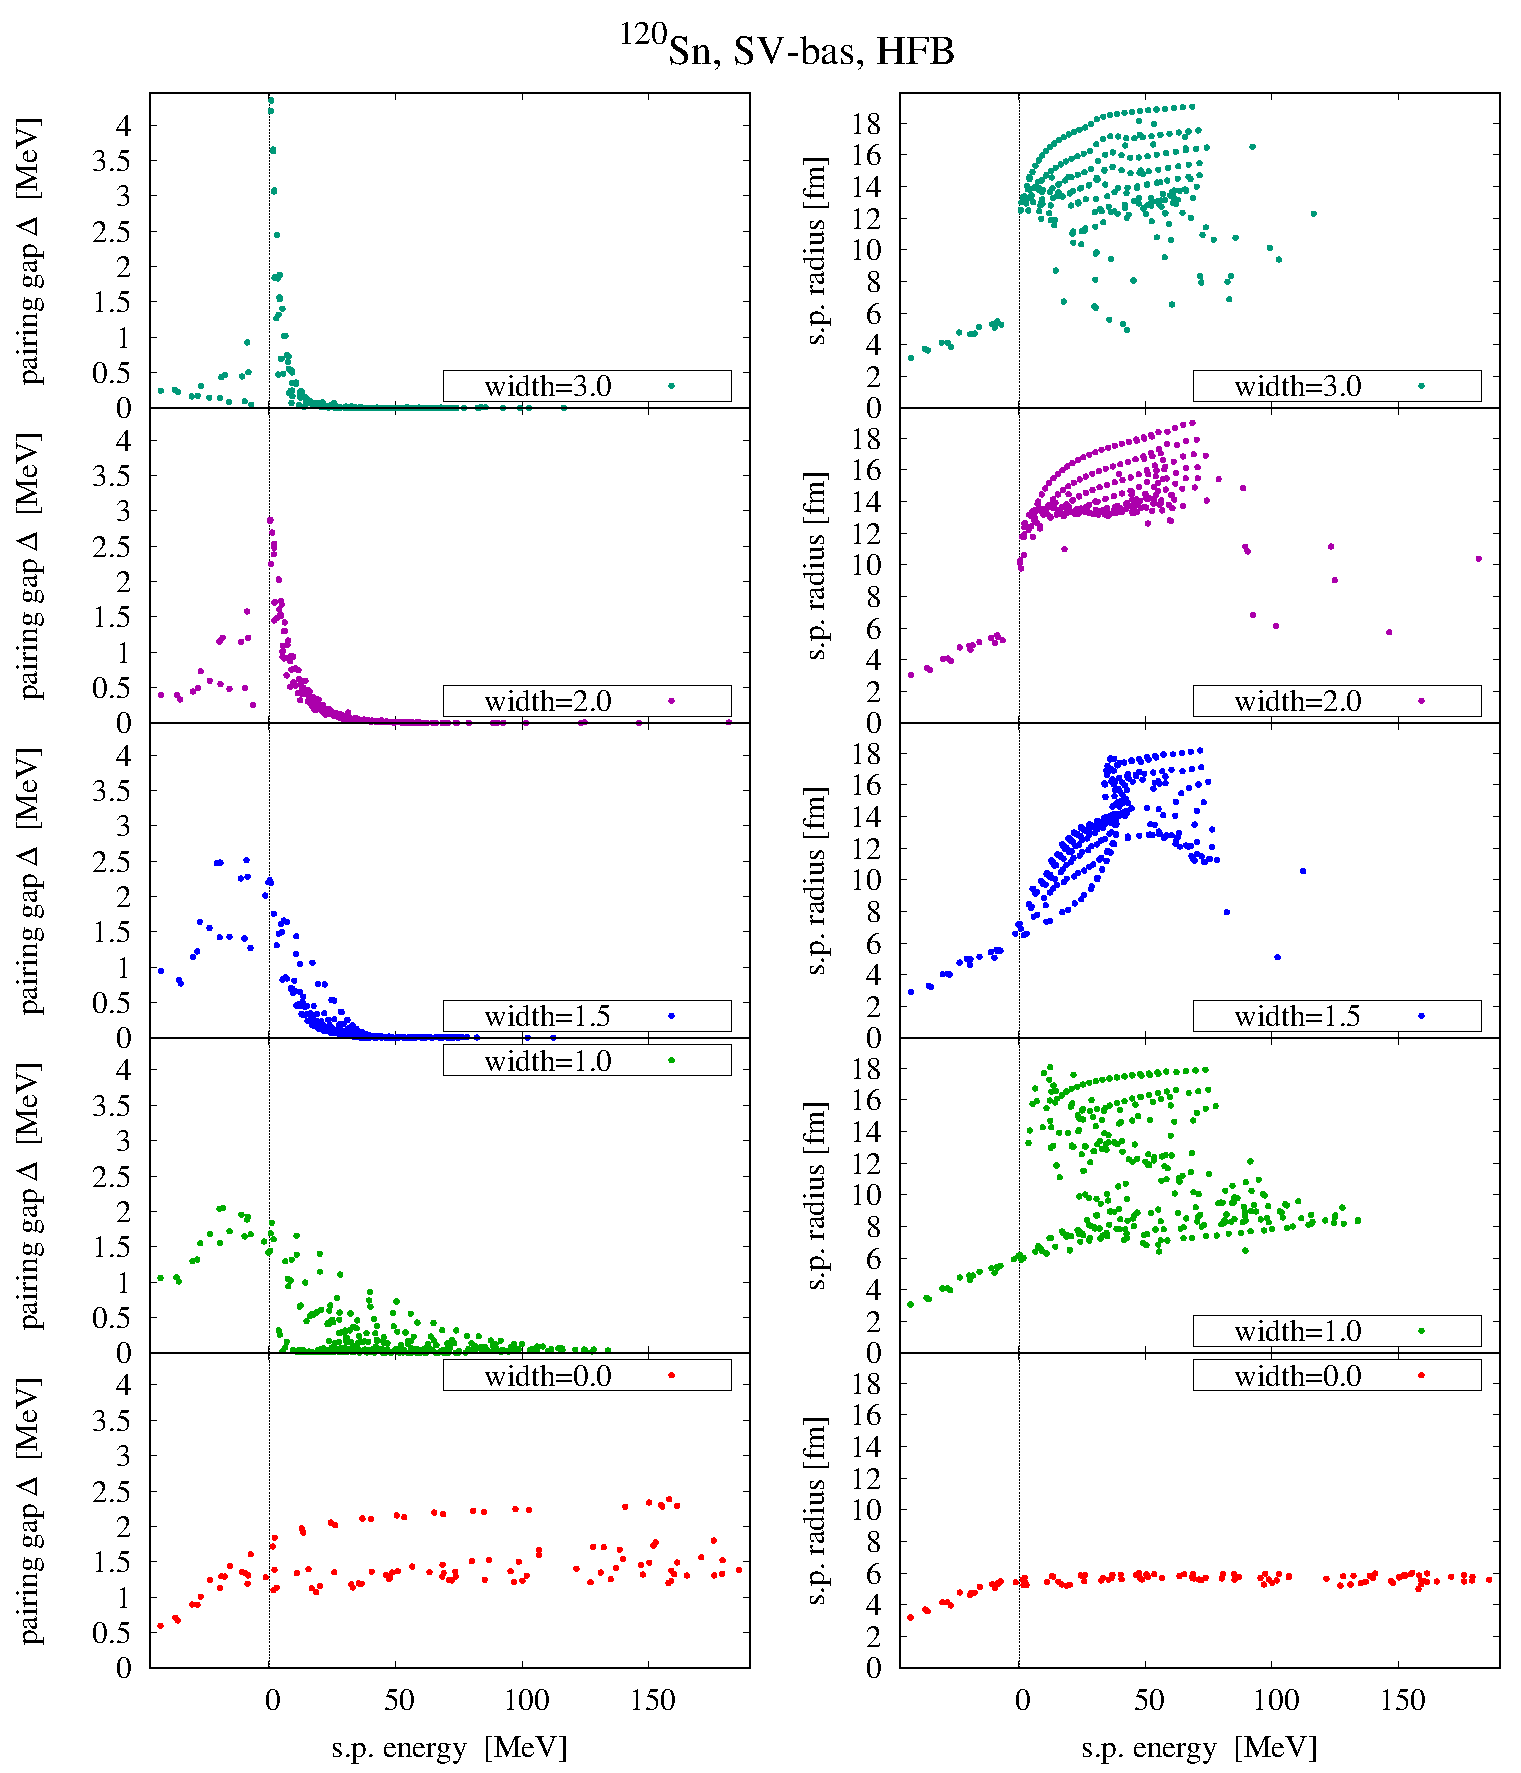
\includegraphics[width=0.8\linewidth]{varywid_HFB}}

\bigskip


\end{document}
